% to get nice cover and sections
\documentclass[titlepage]{article}

% margin
%\usepackage[margin=1.5cm]{geometry}

% to use images
\usepackage{graphicx}

% use spanish
\usepackage[spanish]{babel}

% bibliography manager
\usepackage[style=alphabetic]{biblatex}
\addbibresource{refs.bib}
\usepackage{csquotes}

% motseratt font is nice, but doesn't have math symbols
% Fira math seems ok to replace them
\usepackage{fontspec}
\setmainfont{montserrat}
\usepackage[mathrm=sym]{unicode-math}
\setmathfont{Fira Math}

% simple UML diagrams
\usepackage{plantuml}

% nicer links
\usepackage{hyperref}
\usepackage{cleveref}

% cover info
\author{Edgar Quiroz}
\date{\today}
\title{
  Mejoras a AEL\\
  Diseño de Interfaces de Usuario
}

\begin{document}

\begin{titlepage}
\maketitle
\end{titlepage}

\section{Contexto y uso de la aplicación}
La Aplicación web para el proceso Educativo sobre el Logaritmo  (AEL)
desarrolada en \cite{Salas-Rueda_2020} calcula detalladamente el tiempo (número
de años) durante la solicitud de un crédito bancario. La interfaz gráfica actual
se puede ver en la \cref{img:ael}. Basado en la descripción original y en los
criterios dados en \cite{req}, el contexto de uso es el siguiente.

\begin{figure}
\centering
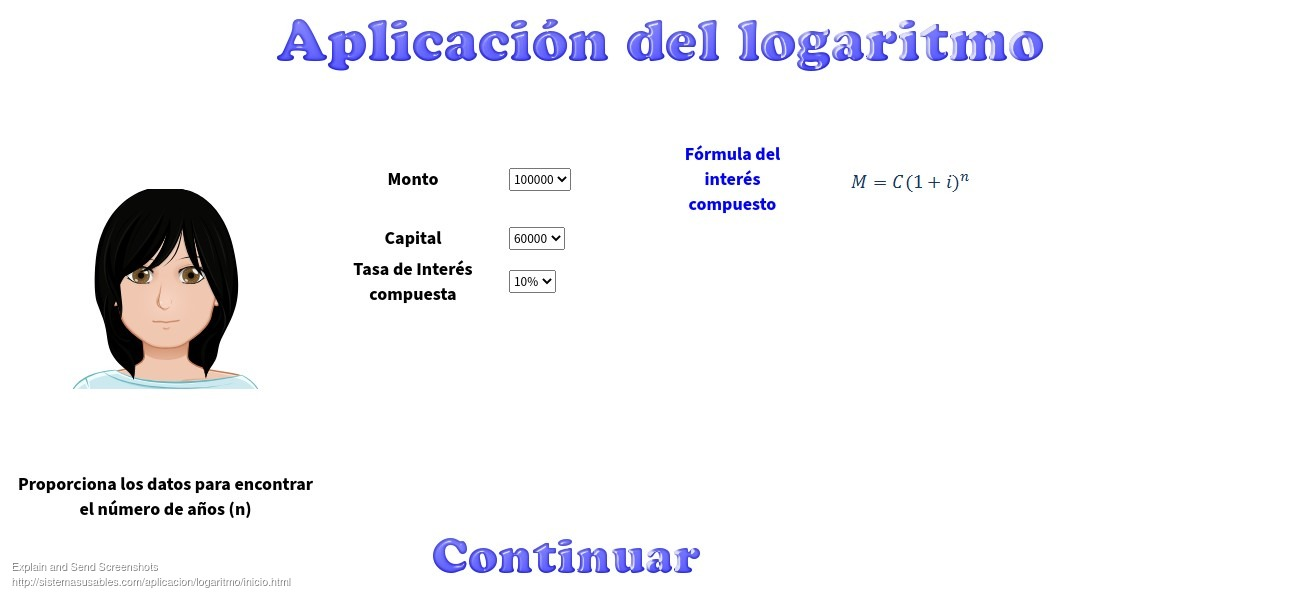
\includegraphics[scale=0.25]{./imgs/ael_inicio.jpg}
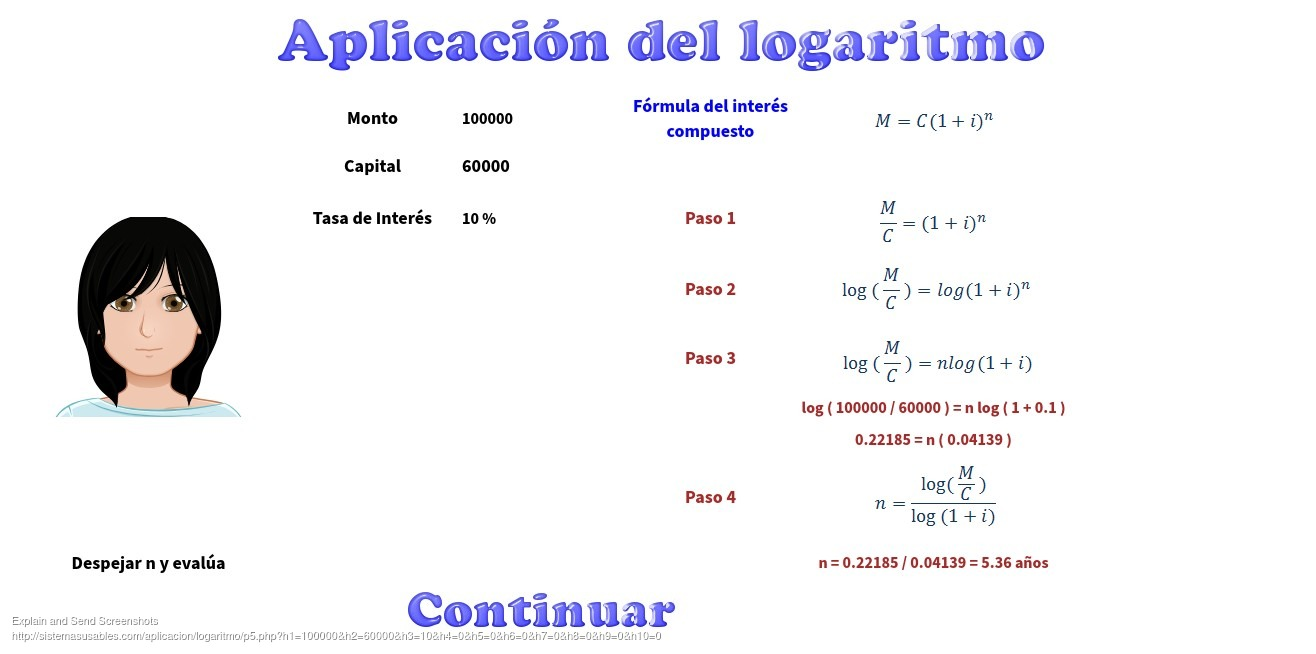
\includegraphics[scale=0.25]{./imgs/ael_fin.jpg}
\caption{Diseño actual de AEL}
\label{img:ael}
\end{figure}


\begin{itemize}
  \item Funcionalidad: el sistema mostrará paso a paso el cálculo del tiempo
        necesario para calcular un interés compuesto con un monto objetivo,
        capital inicial e interés dados por el usuario. Como es un sistema
        interactivo, el tiempo de respuesta debe ser lo menor posible.
  \item Usuarios: habrá un único tipo de usuario (alumnos), que solo deberían
        tener experiencia básica en uso de computadoras.
  \item Documentación: no se requiere documentación más que este documento.
  \item Datos: la entrada y salidad de datos es únicamente a la interfaz
        gráfica, y el formato de presentación es libre. El cálculo de las
        operaciones se podría pedir con la precisión de día (aproximadanete
        cuatro figuras después del punto). La cantidad de datos a procesar es
        mínima. Una decena de usuarios con un conjunto de datos sería lo más a
        usar. No es necesario guardar ningún tipo de información.
  \item Seguridad: no es necesario controlar el accesso. Como no hay información
        a guardar, no es necesario proteger nada.
\end{itemize}

Como solo hay un usuario y el sistema tiene un solo requerimiento funcional,
habrá un único caso de uso para mostrar los pasos del cálculo del interés. Un
esquema \emph{UML} de este caso se puede ver en la \cref{uml:ael-usecase}.

\begin{figure}
  \centering
  \begin{plantuml}
    @startuml
    !theme plain
    left to right direction
    actor estudiante
    rectangle AEL {
      usecase (Visualizar cálculo de interés compuesto) as viz
    }
    estudiante --> viz
    @enduml
  \end{plantuml}
  \caption{Caso de uso para AEL}
  \label{uml:ael-usecase}
\end{figure}

\section{Perfil de los usuarios}
La muestra original son 29 alumnos que cursaron la asignatura Matemáticas
Básicas en una universidad mexicana durante el ciclo escolar 2015. Estos alumnos
cursaron el primer semestre de las carreras en Administración ($n=7, 24.14\%$),
Contaduría ($n=5, 17.24\%$), Comercio ($n=11, 37.93\%$) y Mercadotecnia ($n=6,
20.69\%$).

Como no se tiene acceso a más información de los usuarios originales, se usarán
datos obtenidos de \cite{PEU}.

\subsection{Mapas de empatía}

\subsection{Artefactos de persona}

\section{Navegación}

\section{Wireframes}

\section{Color}

\section{Interactividad}

\section{Pruebas de usabilidad}

\printbibliography

\end{document}
